\chapter{Pilot placement method using Deep Q-Learning}\label{ch:channel_q_learning}


The importance of \gls{csi} data for transmission optimization have been outlined and described in Chapter \ref{ch:pilot_sequence}. Several techniques for improving channel estimators have been detailed in Chapter \ref{ch:channel_estimation}. These techniques utilise both the statistics obtained from the channel, but the pilot placement. In this chapter, a novel solution for pilot optimisation is presented. The method uses Deep Q-Learning to optimise the placement of the pilots. The chapter will be structured as follows. Section \ref{sec:optimal_pilot_placement} will introduce the problem of optimal pilot placement and the resulting approach of the proposed method. Section \ref{sec:reinforcement_learning_principles} will introduce the terms associated with deep reinforcement learning. Section \ref{sec:interactive_environment} will contain a description of the simulation environment and the required parameters and furthermore detail the implementation requirements.  Section \ref{sec:RL_results} will present the results of the proposed method and is extended by the discussion in Section \ref{sec:RL_discussion}. A conclusion is presented in \ref{sec:RL_conclusion} and a compressed summary is given in \ref{sec:RL_summary} along with the most important challenges faced.

The content of this chapter largely corresponds to the work published in \cite{Thrane2020PilotQ-Learning}. However, this chapter extends the published results and the necessary discussion in an attempt to identify future opportunities. 





\section{Optimal pilot placement}\label{sec:optimal_pilot_placement}
\begin{figure*}
    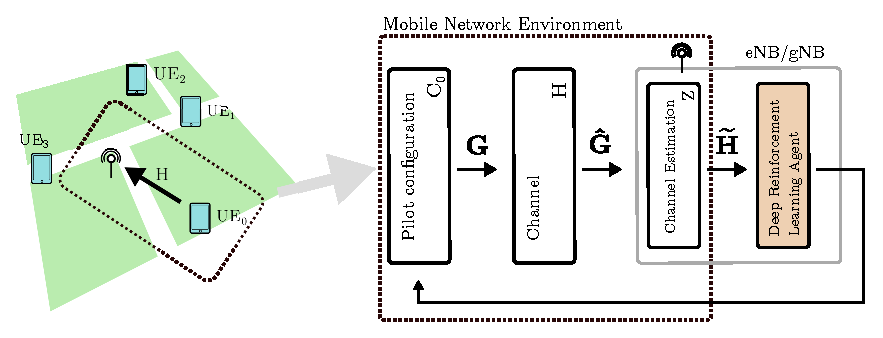
\includegraphics[width=\textwidth]{chapters/part_uplink/figures/RL_introduction_maindrawing.eps}
    \caption{The user transmits a pilot sequence over the air to the \gls{enb}. The channel estimation accuracy is directly related to the interference caused by other users in the environment, but also the placement of the pilots.}\label{fig:RL_introduction_maindrawing}
\end{figure*}
When employing the so-called \gls{srs} sequences in uplink transmission, several optimisation issues arise. Most significantly, 1) ideal pilot placement given the channel estimator function and the statistics, 2) Avoiding inter-cell interference between non-orthogonal pilot configurations (see chapter \ref{ch:pilot_sequence} for \emph{pilot contamination}) . So in other words, the placement of the pilots needs to consider the channel estimator and the channel statistics but also interfering source, e.g. other users and their respective configuration. The placement of the \gls{srs} sequence turns into a complicated optimisation problem that requires fundamental knowledge of two complex situations, the channel conditions and the users in the radio environment. 

The authors in \cite{Simko2013AdaptiveSystems} design an ideal placement strategy which is derived using the auto-correlation function of the channel. Obtaining this function is in practice, not a feasible operation, and shares many similarities with the \gls{mmse} channel estimator as shown in chapter \ref{ch:channel_estimation}. The primary purpose of the novel solution presented in this chapter is to avoid the need for this auto-correlation function and learn all necessary statistics through iterative learning of interacting with the radio environment. 



We consider a mobile environment to consist of multiple users within a given cell, as visualised in Fig \ref{fig:RL_introduction_maindrawing}. Each user has a corresponding pilot configuration which, in practice, is defined as outlined in Section \ref{sec:srs_sequence_definition}. The channel imposed on each transmitted pilot sequence is then a result of:  1) physical interactions, e.g. common radio impairments of large-scale and small-scale fading (see chapter \ref{ch:channelmodellingbasics}). And 2) other users the interference caused by overlapping sequences (as visualised in Fig. \ref{fig:RL_srs_configuration_overlap}. Furthermore, this might be enhanced by neighbouring cells and the respective users within. The channel imposed on the transmitted pilot sequence is thus complex and consists of several intractable factors. 

\begin{figure}
    \centering
    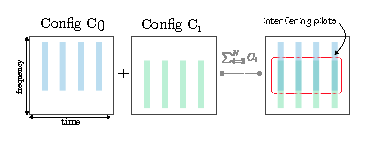
\includegraphics{chapters/part_uplink/figures/RL_srs_configuration_overlap.eps}
    \caption{The limited adaptability of \gls{srs} configurations can result in non-orthogonality between pilots.}\label{fig:RL_srs_configuration_overlap}
\end{figure}


\subsection{Common notations}
A few notations are required to formalise the problem and the proposed method. The notations are similar to the content on Chapter \ref{ch:channel_estimation}. The spatial and temporal domain of cellular systems such as LTE and \gls{nr} operate in frequency and time with distinct definitions of frequency and time components. In other words, frequency is defined in terms of the number of \gls{ofdm} subcarriers. While time is defined in terms of \emph{subframes} corresponding to a duration of $1$ ms. In this particular case we define a number of \gls{ofdm} subcarriers of past $m$ subframes with bold: $\mathbf{H} = H[t],H[t-1],...,H[t-m]$. where $t$ denote the subframe and thus $t - m$ denote the time of $m$ subframes prior. Additionally, capital letters (such as $H$) is considered in the frequency domain. We introduce a few notations and definitions as follows

\begin{itemize}
    \item $H_j$ frequency response for a time-variant channel for some user $j$
    \item $G_j$ is the generated and transmitted \gls{srs} sequence for some user $i$ with configuration $C_j$ and bandwidth $W$
    \item $\hat{G_j}$ is the received and demodulated \gls{srs} sequence for some user $j$
    \item $\widetilde{H_j}$ is the estimated channel response for some user $j$
\end{itemize}

Visual examples of both, $H_j$, $\widetilde{H_j}$, $\hat{G_j}$ can be seen in Chapter \ref{ch:channel_estimation}, more specifically Fig. \ref{fig:prediction_example_grid}. Using these notations we can define $\hat{\mathbf{G_j}}$ as a function of the time-variant channel and the \gls{ici} present in the radio environment. This is seen in Eq. (\ref{eq:received_signal_model})
\begin{equation}\label{eq:received_signal_model}
    \hat{\mathbf{G_j}} = \mathbf{G_j} \cdot \mathbf{H_j} + \overbrace{\sum_{j \neq i}^N \mathbf{G_j} \cdot \mathbf{H_j}}^{ICI} + \epsilon
\end{equation}

The estimated channel can then be denoted as follows:
\begin{equation}\label{eq:channel_estimation_function}
    \widetilde{\mathbf{H_j}} = Z(\mathbf{\hat{G_j}}) 
\end{equation}

Where $Z(\cdot)$ is the channel estimator function as detailed in Section \ref{sec:channel_estimators}. It can be seen from Eq. (\ref{eq:received_signal_model}) and (\ref{eq:channel_estimation_function}) that the channel estimation quality is corrupted by the magnitude of \gls{ici} and measurement noise $\epsilon$. The channel estimation is thus not only an estimation of channel characteristics but also the interfering pilot signals contaminating the radio environment.

\section{Reinforcement Learning principles}\label{sec:reinforcement_learning_principles}
The subject of reinforcement learning contains many principles and terms which can be confusing to the novice. This section will thus contain a summary of the essential terms required for the fundamental understanding of how reinforcement learning works. Deep Q-learning is the use of Deep Learning methodologies in combination with reinforcement learning principles; thus, the tool is considered deep reinforcement learning. The area of deep reinforcement learning has gained a lot of attention due to recent work such as a computer learning to play Atari games \cite{MnihPlayingLearning}, defeating world champions in complicated games such as Go \cite{Silver2016MasteringSearch} and recently destroying players in Starcraft II \cite{Vinyals2019GrandmasterLearning}. Deep Reinforcement Learning has revolutionised control and information theory by being capable of predicting the most likely future states given billions of possible states without actually having to compute all combinations.

Being capable of mapping a state to an action to maximise a reward is the essence of reinforcement learning. The performance of reinforcement learning systems is heavily based on the quality of the feature representation. Deep Learning systems are capable of extracting high-quality features from high dimensional data (as also illustrated in chapter \ref{ch:satelliteImages}). In essence, it is the same paradigm applied to reinforcement learning problems. However, a few challenges exist. More noticeably the data quantity in reinforcement environments is significantly less than required in other deep learning applications. For example, state of the art deep learning algorithms have learned from large amounts of data which is not the case in reinforcement learning situations. Reinforcement Learning algorithms learn from a sparse, noisy and delayed reward signal which is quite the opposite from large quantities of data \cite{Sutton2017ReinforcementSecond}. 

The area of Deep Reinforcement Learning uses many principles and definitions. A collection of the essential definitions can be found below


\subsection{Definitions}
\begin{margintable}
    \centering
    \footnotesize{
    \begin{tabular}{l|l}
        Definition & Symbol  \\ \hline
        Reward & $r_i$ \\
        Critic & $Q(s, a)$ \\
        Target Critic & $Q'(s, a)$\\
        Critic Parameters & $\theta_Q$ \\
        Discount Factor & $\gamma$ \\
        Value function target & $y_i$ \\
        Observation & $s$ \\
        Next observation & $s'$ \\
        Action & $a$ \\
        Next Action & $a'$ \\
    \end{tabular}
    \caption{Notation used for Deep Q-learning}
    \label{tab:deep_q_learning_symbols}
    }
\end{margintable}

\paragraph{Episode}
Consists of a finite number of steps and ends at some defined state. For instance, when game over is reached or the end of some predefined sequence of steps. In this case, when a predefined set of scheduling rounds and subframes are completed.

\paragraph{Agent}
The module that learns and acts. The objective of the agent is to maximise a set of rewards by interacting with the environment using a set of predefined actions. Knowing which actions to apply is the objective of the model that the reinforcement learning algorithm is to learn.

\paragraph{Environment}
A system that provides a state responds to actions and offers feedback in terms of rewards. The agent interacts with the environment to learn how states, actions and rewards associate with each other.

\paragraph{Policy}
The mapping of a given state to a specific action. A policy is commonly defined as a lookup table or a function. 

\paragraph{Reward signal}
The goal of reinforcement learning problems. The reinforcement learning model is tasked with maximising the reward and can only influence it through the taken actions.

\paragraph{Value function}
Defines (or approximates) what is best in the long run given the observed state. The value function can be seen as the expected reward for a given state and until the end of the defined episode. 

\paragraph{Q value}
A measure of the overall expected reward given an action $a$ in a state $s$. Denoted as the output measure of the critic function $Q(s, a)$. Similar to a value function, however a slight difference in when the reward is observed. The Q value is a measure of the expected reward of the episode after an action has been taken.


\section{Learning objective}
The purpose of the learning algorithm is two-fold and based on the hypothesis that there exists such a sequence of pilot signals, that is capable of 1) minimising the contamination and 2) improving interpolation methods by strategically placing pilot signals in time and frequency. The algorithm used for this is of type \emph{Deep Reinforcement Learning}, more specifically a \emph{Deep Q-Learning} algorithm. The method utilises a set of neural networks to 1) extract latent information from the radio environment, and 2) interact with the environment. The interaction with the environment is done using a set of predefined actions and a reward function; thus, the main objective is to improve the channel estimation by adjusting the placement of the \gls{srs} sequence. The interaction between placement and channel estimation performance is formalised in terms of maximising rewards over the duration of an episode. Using a Q-learning system the objective is to maximise the expected reward

\begin{equation}\label{eq:bellman-equation}
    y_i = Q(s, a) = r_i + \gamma \text{max}_{a'} Q^{'}(s', a' | \theta_Q')
\end{equation}

Also known as the Bellman Equation (rewritten to use Q values, absolute proof is found in \cite{Sutton2017ReinforcementSecond}) that describes the value of a state as the decomposition of the immediate reward, $r_i$, the next state $s'$ and action $a'$. A discount factor is added, termed $\gamma$, this weights immediate rewards versus long-term rewards and is subject to optimisation. We can rewrite Eq. (\ref{eq:bellman-equation}) to consider the channel estimation for a user $j$  as follows

\begin{equation}\label{eq:value-function}
    y_i = Q(s, a) = r_i + \gamma \text{max}_{a'} Q^{'}(\mathbf{\widetilde{H_{j,i}^{'}}}, a^{'} | \theta_Q')
\end{equation}

The Q value of the current state is determined by 1) the observed reward for a given action, i.e. the reward associated with the placement of a \gls{srs} sequence. And 2) a weighted Q value of the next state given the next action, i.e. a value characterising the \gls{srs} sequence placement that maximises the channel estimation performance. So how do we determine the best action? In other words, how do we determine the best placement of the \gls{srs} sequence? The value function determines the expected reward for a given state. Thus the action that offers the highest Q value is the best action, of course given that the value function is well designed, therefore:

\begin{equation}\label{eq:critic-action}
    a = \arg \text{max}_{a} \; Q(s, a | \theta_Q)
\end{equation}

In other words, for a given set of parameters, the action $a$ that maximises the Q value is the best action which leads back to Eq. (\ref{eq:bellman-equation}). This can be rewritten using the notation for the channel estimation for a specific user $j$ as follows.

\begin{equation}\label{eq:critic-action}
    a = \arg \text{max}_{a} \; Q(\mathbf{\widetilde{H_{j}}}, a | \theta_Q)
\end{equation}

What this intuitively means is that the observation of the channel estimation shall offer a Q value that determines the best pilot sequence placement. The best pilot sequence placement being learned through the reward function. If the reward function is designed to optimise future channel estimation error, the action, e.g. the pilot sequence placement, will thus be an action that improves future channel estimation.

\subsection{Actions}
An action is defined as a set of inputs that are given to the environment. It is thus the only way for the \emph{agent} to interact with the environment. In this particular case, the pilot sequence positioning is the only thing the agent is capable of adjusting. The well-defined standards of LTE and NR (as described briefly in Section \ref{sec:srs_sequence_definition}) allows for a direct mapping to a finite set of actions. The action space of \gls{srs} sequences, can be found to be rather complicated; therefore, the action space, i.e. the configuration of the pilot sequence is simplified. The position in frequency is the only free parameter that can be adjusted and is reduced to the following: 

\begin{equation}
   a \in [0, 1, 2, ..., 9]
\end{equation}

Where each integer denotes a starting position in frequency (i.e. subcarrier index) which is ultimately determined by the bandwidth allocated to the \gls{srs} sequence. The bandwidth is split into $M$ parts, and this means the starting position can be translated into a subcarrier index using the following:

\begin{equation}
    F_{pos} = M \cdot a
\end{equation}

Where $M$ can be computed as $(\text{NULRB} \cdot 12) / |a| = M$ where $|a|$ is the total number of actions available. 

\subsection{Reward function}

Designing the reward is essential to the effectiveness of the reinforcement learning agent \cite{Sutton2017ReinforcementSecond}. In this particular work, an \emph{extrinsic} reward is used due to the simplicity. However, state of the art argues that \emph{intrinsic} rewards result in improved results and stability of the learning process \cite{SinghIntrinsicallyLearning} due to the improved exploration properties. The discussion of extrinsic rewards and intrinsic rewards is beyond the scope of this dissertation. The simplistic extrinsic rewards outweigh the difficulties and complex features of intrinsic rewards for the problem presented. 

The \gls{mse} metric is used for measuring the channel estimation accuracy. Thus, the estimation accuracy is measured using the true channel conditions. The \gls{mse} of the channel estimation for a given state $s$, at a given time $t$ for a given user $j$ is formalized using Eq. (\ref{eq:sum-of-squares}), e.g.

\begin{equation}\label{eq:mse_channel_estimation}
    \text{MSE}_{j,t} = \frac{1}{N} \sum_{k = 0}^{N} ( |\mathbf{H_{k,j}}| - |\mathbf{\widetilde{H_{k,j}}}| )^2
\end{equation}

Where $k$ and thus $N \in H_{n \times m}$ is used as the index of the matrix. The \gls{mse} is formalised as the absolute error squared between the channel estimation and the true channel conditions. This metric of error is used for the design of the reward function. The reward function being the reason that the \emph{agent} learns which actions improve channel estimation. The reward is then formalised as the difference in the channel estimation error between a current state and the next state, or the current state and the previous state as follows

\begin{equation}
    \Delta \text{MSE}_j = \text{MSE}_{i,t} - \text{MSE}_{i,t+1}
\end{equation}

The intuition here is that taking an action that improves the channel estimation for the next step offers a positive $\Delta$ value, as the error is lower than previous. This means that the reward can be designed around the nominal difference in \gls{mse}. In other words, taking an action that increases the error between the channel estimation and the true channel conditions returns a $\Delta \text{MSE}$ value that is negative. Several reward functions can be formalized using the error difference (which is also known as a extrinsic reward function). A reward function that heavily penalize wrong decisions can be defined as:

\begin{equation}\label{eq:reward_minus_5}
r(\Delta \text{MSE}) = \begin{cases}
1 &\Delta \text{MSE} >= 0\\
-5 &\Delta \text{MSE} < 0
\end{cases}
\end{equation}

\noindent And a less heavy penalty

\begin{equation}\label{eq:reward_minus_1}
r(\Delta \text{MSE}) = \begin{cases}
1 &\Delta \text{MSE} >= 0\\
-1 &\Delta \text{MSE} < 0
\end{cases}
\end{equation}

\begin{figure}
    \centering
    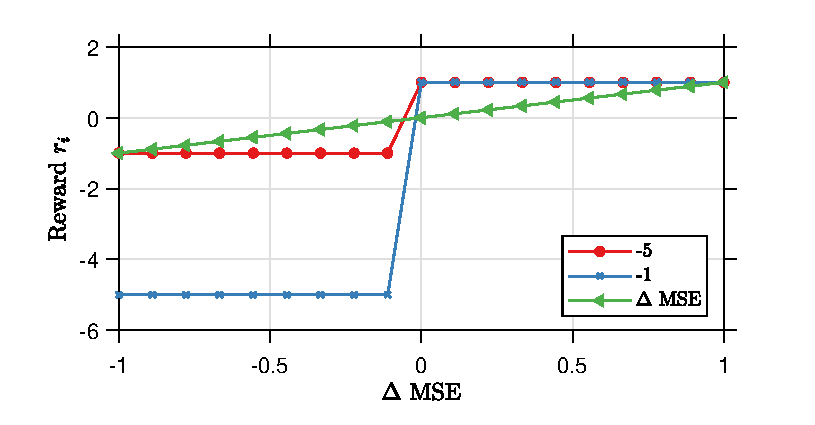
\includegraphics{chapters/part_uplink/figures/reward_example_figure.eps}
    \caption{Using the error difference directly results in a linear reward. Using a step function such as Eq. (\ref{eq:reward_minus_5}) simplifies the learning.}
    \label{fig:reward_example_figure}
\end{figure}

The result of both will be presented, and a discussion will follow later in this chapter. However, before doing so, the Deep Learning model and the subsequent steps of the Deep Q-learning algorithm will be summarised and outlined.

\subsection{Deep Q-network}
The critic network, or the \emph{Deep Q-network} provides with the Q values for learning. Deep Learning principles have been shown before to be capable of handling data with high dimensionality. The principles and methods of Deep Learning can be translated to Q-Learning, and thus the name Deep Q-Learning. The purpose of the critic network is to learn through observations of the current environmental state which action maximises the expected reward as noted by Eq. (\ref{eq:bellman-equation}). In other words, by observing \gls{csi} data and adjusting the placement of the \gls{srs} sequence the expected reward (the channel estimation performance) is to be maximised. Using methodologies of Deep Learning Models, the model can essentially be constructed as a Deep Learning model which we from this point on term a \gls{dqn}. Shown in Chapter \ref{ch:channel_estimation}, convolutional layers have shown to be effective at dealing with raw \gls{csi} data, which is the main heuristic followed in the design of the \gls{dqn}. Through the nonlinear transformations of the \gls{dqn}, the raw \gls{csi} data is transformed, using updated parameters into useful latent information. The parameters of the critic network is updated using principles of backpropagation and require a loss function. If the reader can recall, an example of such a loss function is the common sum-of-squared error function Eq. (\ref{eq:sum-of-squares}). The loss function used in this work, utilise the sum-of-squared error and can be rewritten using terms and notations relevant, which results in Eq. (\ref{eq:critic-loss})

\begin{equation}\label{eq:critic-loss}
     L = \frac{1}{M} \sum_{i=1}^M(y_i - Q(\mathbf{\widetilde{H_{j,i}}}, a| \theta_Q)^2)
\end{equation}

\noindent Two sets of parameters for the Deep Q-Learning method is required. A critic, and a \emph{target} critic. The purpose of having both is essentially a requirement for optimising the critic network offering the Q-values. This can be seen from Eq. \ref{eq:bellman-equation} where the maximisation of future rewards is dependent on the same parameters that are attempted to be learned. By using a separate set of parameters, it offers an iterative process of updating the parameters. The parameters of the target critic are updated using:

\begin{equation}\label{eq:critic-target}
    \theta_{Q'} = \tau \theta_Q + (1-\tau ) \theta_{Q'}
\end{equation}

\noindent Where $\tau$ is a smoothing parameter that assists in the stability and convergence of iterative learning. In other words, the parameters of the target \gls{dqn} are updated using a decomposition of the current critic parameters and the target critic parameters. The parameters of the target critic (noted $\theta_{Q'}$) are updated using the parameters of the critic (noted $\theta_Q$). In summary, 

\begin{enumerate}
    \item The weights of the critic network is updated using backpropagation wrt. $\theta_Q$ and the loss in Eq. (\ref{eq:critic-loss})
    \item The target critic is updated using Eq. (\ref{eq:critic-target})
\end{enumerate}

\subsection{Discount factor}
The discount factor $\gamma$ in Eq. (\ref{eq:bellman-equation}) represents how future rewards are discounted. If close to $0$, immediate rewards are pursued, while if close to $1$, long-term future rewards are pursued. The equation defines the discounted rewards for a given state sequence, for each of which a reward is observed. The discount factor can also be seen as the "impatience" factor. A $\gamma = 1$ offers only additive rewards while $\gamma = 0$ use the immediate reward of the current state. 

\subsection{Greedy Exploration}
At the end of each training step, if $\epsilon$ is greater than $\epsilon_{min}$, then it is updated with $\epsilon = \epsilon (1-\alpha_{\epsilon}$). Where we defined $\epsilon$ as the probability threshold to select an action randomly from a uniform distribution or select the action that maximises the state-action value function. This approach is to ensure the model explores the state space, as maximising the long-term rewards might include actions that do not explicitly improve the next channel estimation.




\subsection{DQN algorithm}\label{subsec:dqn_algorithm}
\begin{figure}
    \centering
    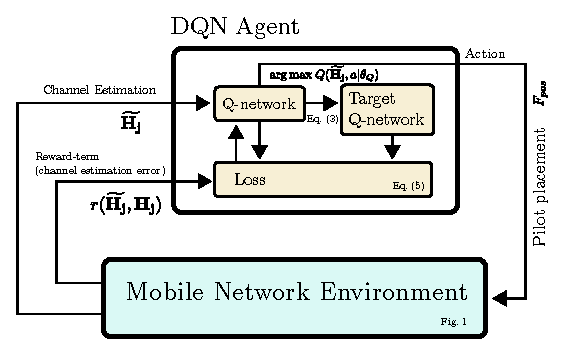
\includegraphics[width=\textwidth]{chapters/part_uplink/figures/RL_dqn_architecture_simplified.eps}
    \caption{Flow of the \gls{dqn} architecture}
    \label{fig:dqn_architecture_simplified}
\end{figure}

The algorithm for the \gls{dqn} can be summarized as visualized in Fig. \ref{fig:dqn_architecture_simplified}, and as follows: 


\begin{enumerate}
    \item Observe $\mathbf{\widetilde{H_j}}$ from the environment and select a random action $a$ with probability $\epsilon$. Otherwise select an action provided by the \emph{critic value function} Eq. \ref{eq:critic-action}.
    \item Execute the action $a$ and observe the reward $r$ along with the next observation $\mathbf{\widetilde{H_j^{'}}}$
    \item Store this experience in a buffer (memory replay)
    \item Sample a mini-batch of $M$ experiences from the buffer
    \item If the observation $\mathbf{\widetilde{H_j^{'}}}$ is a terminal state the value function is set to $r$ otherwise we use Eq. \ref{eq:value-function}
    \item Update parameters of the critic network using the loss function in Eq. \ref{eq:critic-loss} and the gradient wrt. 
    \item Update the target critic using Eq. \ref{eq:critic-target}
\end{enumerate}

This is repeated until the terminal state is reached.

\section{Model architecture}
The Q-network consists of several layers and modules, as visualised in Fig. \ref{fig:rl_q_network}. The Q-network is split into three paths for handling: 1) the observations, 2) the actions, and 3) the output. 

\paragraph{The \textbf{observation path}} denotes the use of a convolutional neural network where $\widetilde{\mathbf{H_j}}$ is given as input. The objective of this path is to extract necessary information from the channel estimation that can aid in the learning process. The input size is of $N \times T \times C$ where $N$ is the number of subcarriers, $T$ is the number of subframes, e.g. \gls{ofdm} symbols and $C$ is the number of channels (real and imaginary part of the channel estimation). A sequence of three convolutional blocks is used each with a stride of $[2, 2]$ and no maximum pooling operation. The \textit{\gls{relu}} activation function is used between the layers. Each layer considers 40 filters, each with the corresponding kernel size: $[5,5], [3,3]. [2,2]$. 

\paragraph{The \textbf{action path}} denotes the use of a 2-layer \gls{nn}. The \gls{nn} is to be capable of learning any complex interactions between the choice of an action and a given observation. A fully connected linear neural network is used, with no activation function. 

\paragraph{The \textbf{output path}} considers the combination of the action path and the observation path to enable the learning of any complex interactions. A single-layer \gls{nn} with $30$ neurons and no activation function is used. The input is given as the sum of the output of the action path and the observation path. The output of the \textbf{output path} provides with the Q value used for the \textit{value function}. 

\begin{figure}
    \centering
    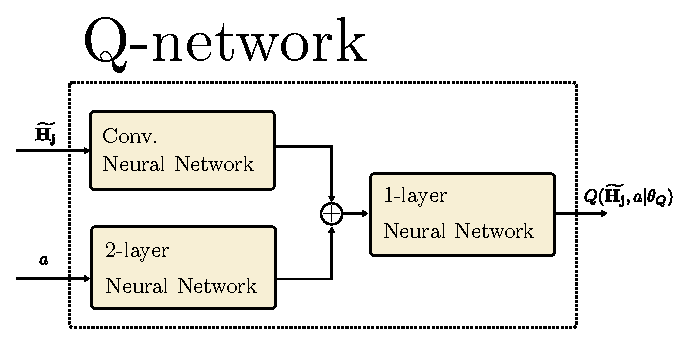
\includegraphics{chapters/part_uplink/figures/RL_Q_network.eps}
    \caption{The Q-network considers 3 submodules. One for observations, one for actions and one for the Q value output.}
    \label{fig:rl_q_network}
\end{figure}


\section{Interactive Environment}\label{sec:interactive_environment}
Reinforcement learning requires interactions with an environment that provides observations, change based on actions and offer feedback for the given action. Efficient implementations of these environments is a necessity and are subject to much research. Several computational tricks are needed for complex systems \cite{Hafner2017TensorFlowTensorFlow}, as a slow learning process significantly hinders progress in terms of model structure and reward functions. In this particular work, the environment has considerable complexity due to the multi-user channel conditions and interference computations. However, a few tricks can be applied as described in this section.

\subsection{Mobile communication system emulator}
The mobile communication system shown in Fig. \ref{fig:RL_introduction_maindrawing} require a channel model for emulating fast and slow-fading impairments. It must also be capable of computing the interference of the pilot sequences between the users in the cell. Moreover, the system needs to be capable of responding within the time resolution used in such systems. The use of the \gls{srs} sequence (and optimisation hereof) provides us with the time scale required. The observations of the channel estimation is a response to a given \gls{srs} sequence and must thus share the time scale of the \gls{srs} sequence. In other words, the observation is defined with time steps of the \gls{srs} sequence, which (if the reader can recall from Section \ref{sec:srs_sequence_definition}) at minimum $1$ ms, and at most $10$ ms. It seems fair that the system operates using standard principles such as subframes ($1$ ms) and full frames ($10$ subframes e.g. $10$ ms) present in \gls{lte} and \gls{nr} systems. Due to the nature of the \gls{srs} sequence, the channel estimator used must consider the \gls{ofdm} symbols where no pilots signals are placed. As recalled from Section \ref{sec:srs_sequence_definition}, the pilot symbols are placed on the last \gls{ofdm} symbol of the used subframe. 


\subsection{Implementation}
First and foremost, the implementation must offer feasible computational run-time for training such \glspl{nn} in an iterative manner. Moreover,  scanning the hyper-parameters, as we saw in Chapter \ref{ch:satelliteImages} requires an extensive amount of experiments. Initially, the task of the environment was to compute all necessary elements during training. For example, emulating the channel conditions, computing interference and doing the channel estimation. It was quickly discovered that this introduced a computational bottleneck and unfeasible run-times. Instead, the channel conditions were precomputed for a finite number of subframes and then loaded into the system. Since the placement of the \gls{srs} sequence change the magnitude of interference, the interference computation must remain in the system and cannot be precomputed. The alternative (precomputing all possible combinations) was deemed not feasible for implementation. The implementation flow is visualised in Fig. \ref{fig:environment_implementation}. The DQN algorithm is implemented with MathWorks MATLAB \cite{MATLABRL_toolbox}. 
\begin{figure*}
    \centering
    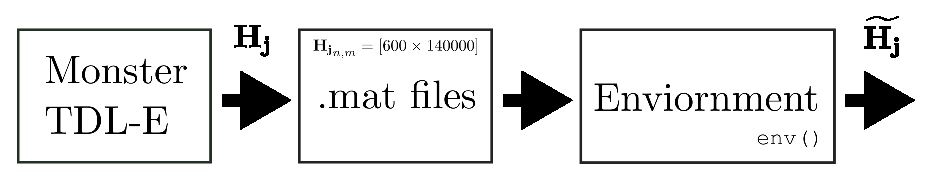
\includegraphics{chapters/part_uplink/figures/environment_implementation.eps}
    \caption{Channel conditions are simulated over $M$ frames and stored. The environment is tasked with loading, computing interference and channel estimation.}
    \label{fig:environment_implementation}
\end{figure*}

Firstly, the channel conditions are obtained (loaded) upon creation of the environment. This prepares the channel conditions and can, therefore, be accessed for each subframe, i.e. iteration. The implementation of the environment follows a sequence of steps. In other words, a sequence of operations is applied at each subframe for data processing that is not directly related to the Q-learning algorithm. Additionally, we can refine the \emph{episode} term to use relevant terms from cellular systems. We define an \emph{episode} as $1000$ frames of an LTE system. The iterations of the system follow the subframe terminology, which means that $10000$ subframes are iterated. The sequence for each iteration can then be outlined as follows:

\begin{enumerate}
    \item Access the channel conditions $H_j$ for each user $j$.
    \item Sample the channel conditions using the \gls{srs} configuration $C_j$ (determined by the action $a$) to obtain $G_j$.
    \item Compute the received \gls{srs} sequence using Eq. (\ref{eq:received_signal_model}) using $H_j$ from interfering users to obtain $\hat{G_j}$.
    \item Add $\hat{G_j}$ to a FIFO for channel estimation.
    \item Estimate the channel using Eq. (\ref{eq:channel_estimation_function}) spatially and temporally using a linear channel estimator.
    \item Execute the Q-learning algorithm following Section \ref{subsec:dqn_algorithm}.
\end{enumerate}

\subsection{Emulation parameters}
The channel model used for emulating fast-fading impairments is determined on a set of parameters. The parameters, e.g. delay-profile and the delay spread can be seen in Table \ref{tab:sim_param}. The implementation is completed using the \gls{monster} library as described in chapter \ref{ch:monster}. 

\begin{margintable}
\centering
\footnotesize{
\begin{tabular}{l|l}
\toprule
\textbf{Parameter}                 & \textbf{Value} \\ \midrule
Carrier frequency $f_c$ & $2.0$ GHz \\
NULRB         & $50$             \\
Delay spread  & $300e-9$         \\
Delay profile & TDL-E          \\
User velocity & $5$ m/s \\   
Number of users & $2$ \\
SRS periodicity & $2$ ms 
\end{tabular}
\vspace{1em}
\caption{Simulation parameters of the channel model and \gls{lte} system configuration}
\label{tab:sim_param}
}
\end{margintable}


\section{Intelligent results}\label{sec:RL_results}
The method is investigated using two distinct experiments to evaluate two essential properties, 1) Learning the channel statistics under the influence of interference and no interference, and 2) Avoiding interference by performing effective actions given the observed channel estimation. The overall parameters used for the Q-learning algorithm is observed in Table \ref{tab:q_learning_param}.

\begin{table}
\centering
\begin{tabular}{l|l}
\toprule
\textbf{Parameter}                 & \textbf{Value} \\ \midrule
\# Training Episodes & $1000$ \\
\# Rounds Per Episode & $200$ \\
$\epsilon$ & $0.3$\\
$\gamma$ & $1e-4$ \\
SINR & $5$ dB (constant) \\
Penality & -5 \\
Interference occupancy & $50\%$
\end{tabular}
\vspace{1em}
\caption{Configuration of training}\label{tab:q_learning_param}
\end{table}

In order to effectively evaluate the properties of the proposed method, the model is trained once and kept fixed, using a fixed set of hyper-parameters and thus weights. The interference is fixed to a constant configuration; such is defined as occupying $50\%$ of the total resources in frequency. The magnitude of \gls{sinr} for these subcarriers is kept constant at $5$ dB. This is to confine the following described experiments, $\mathcal{A}$ and $\mathcal{B}$. 

The reward as a function of scheduling rounds during training, can be observed in Fig. \ref{fig:training_stats_qlearning}. An average reward of $\approx -300$ is observed per episode, consisting of 1000 rounds. This means that on average, $20\%$ of all taken actions during a single episode have resulted in a worse channel estimation. In the case of a decline in channel estimation performance, the reward function provides a penalty of $-5$. 
\begin{figure*}
    \centering
    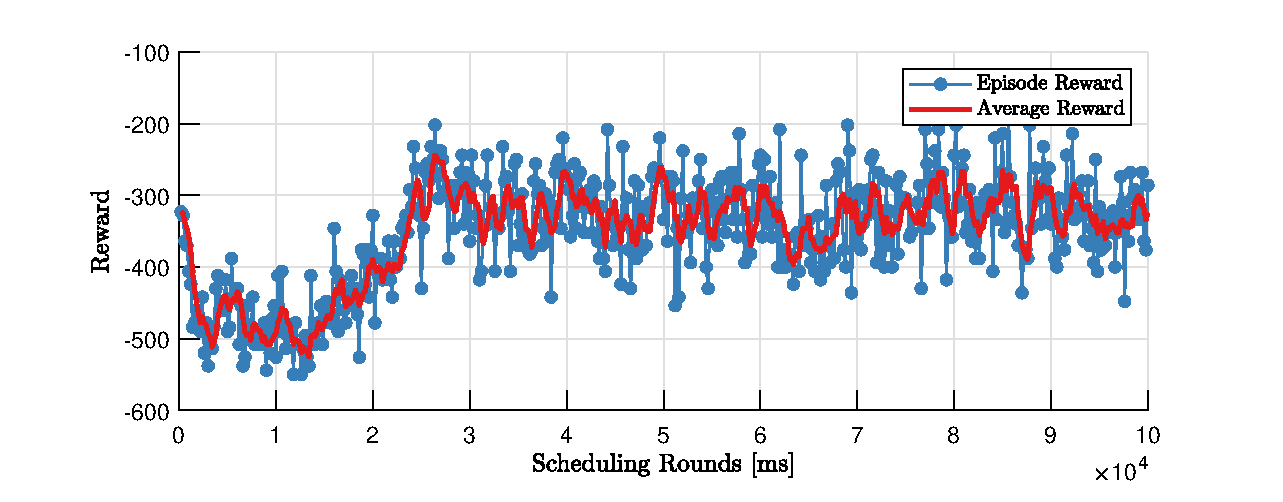
\includegraphics{chapters/part_uplink/figures/results/training_statistics.eps}
    \caption{The reward over the number of scheduling rounds utilised for learning. }\label{fig:training_stats_qlearning}
\end{figure*}
\subsection{Experiments}
Two sets of experiments are defined, $\mathcal{A}$ and $\mathcal{B}$. They differ in terms of added interference. Again, this is to evaluate the trained model using the parameters from Table \ref{tab:q_learning_param}, thus the model is only evaluated (tested) on the two sets of experiments. The evaluation experiments are visualised in Fig. \ref{fig:subcarrier_index_experiment}.


\begin{figure}
    \centering
    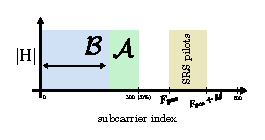
\includegraphics{chapters/part_uplink/figures/subcarrier_index_experiment_setup.eps}
    \caption{The proposed method is evaluate using two seperate }
    \label{fig:subcarrier_index_experiment}
\end{figure}

\paragraph{Fixed interference - $\mathcal{A}$}
The model is trained at a fixed source of interference; however, what happens if the magnitude of interference changes? This experiment seeks to investigate the obtained channel statistics and ensure an optimal solution is not contingent on the interfering source. In other words, the interfering source is kept constant occupying $50\%$ of the available spectrum, but the magnitude of interference in the respective subcarriers is varied.

\paragraph{Dynamic interference - $\mathcal{B}$}
The model is trained on a static and non-realistic scenario. The purpose of this experiment is to evaluate the performance in a more realistic configuration, and more so evaluate the magnitude of generalisation achieved. The interference source is thus changed from being a static interfering source to a secondary user transmitting a similar pilot sequence. The secondary user can adjust the bandwidth of the pilot sequence to explore the proposed method in situations where no interference is present. The bandwidth is adjusted and presented in the results in terms of \emph{\% Interference on available resources}. Such a metric is also considered \emph{pilot contamination}. Several $j$ precomputed channel conditions are utilised for the experiment. The interference is computed using Eq. \ref{eq:received_signal_model}, where each user $j$ have different channel conditions $H_j$. The magnitude of interference, e.g. the \gls{sinr}, is varied to evaluate a difference in spatial positioning of the users.


\paragraph{Test data}
For both evaluation experiments, a separate test set is utilised. The test set differs from the training set with a seed, which offers a difference in channel conditions with the same fundamental parameters and characteristics.

\paragraph{Benchmarking schemes}
To showcase the performance of the proposed method, two simple methods for pilot configuration and thus placement are implemented. These are termed, \emph{static} and \emph{random}. The pilot sequence used in the \emph{static}-scheme utilize a static pilot sequence configuration. In other words, the actions taken by the \emph{static}-scheme is constant and not contingent on \gls{csi} observations. The \emph{random}-scheme uses random actions sampled from a uniform distribution and is thus random over the duration of simulation (again, it is not channel-aware and therefore does not observe any \gls{csi}) 
 \begin{figure}
    \centering
    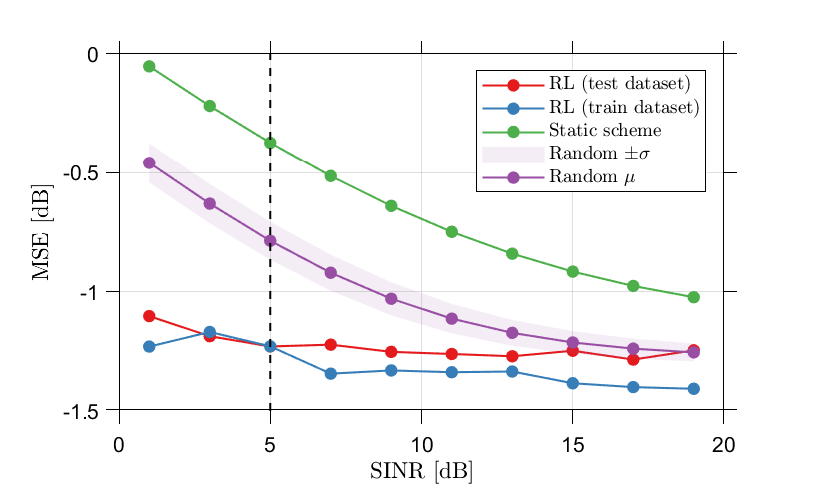
\includegraphics{chapters/part_uplink/figures/results/SINR_sweep.eps}
    \caption{Channel estimation performance (\gls{mse}) as a function of \gls{sinr} evaluted over $1000$ frames.}
    \label{fig:RL_sinr_sweep}
\end{figure}

\subsection{Fixed interference -  $\mathcal{A}$}\label{subsec:RL_results_A}

\begin{figure}
    \centering
    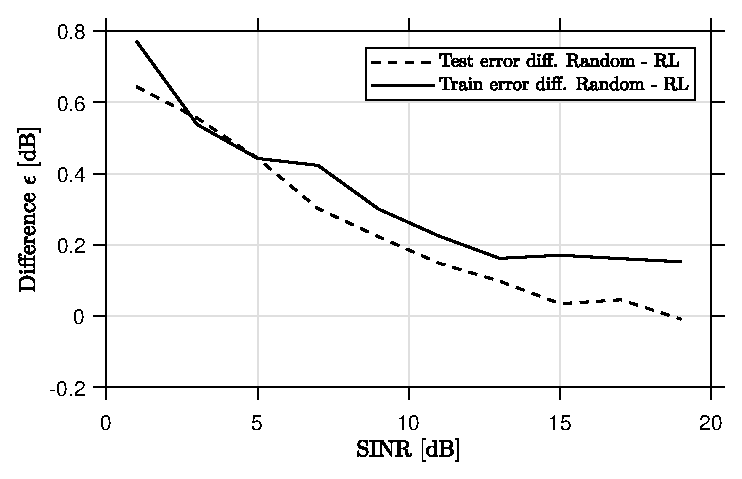
\includegraphics{chapters/part_uplink/figures/results/SINR_sweep_diff.eps}
    \caption{Difference in channel estimation performance (\gls{mse}) between the proposed method and a random selection of pilot positions.}
    \label{fig:RL_SINR_sweep_diff}
\end{figure}
The results of $\mathcal{A}$ can be observed initially in Fig. \ref{fig:RL_sinr_sweep}. The dashed line denotes the magnitude of \gls{sinr} where the model is trained. The \gls{mse} error is the average channel estimation error squared throughout the iterations of the algorithm, as noted by Table \ref{tab:q_learning_param}.  The error of the training and test set are shown to visualise the achieved generalisation. If the reader can recall from chapter \ref{ch:channelmodellingbasics} this is also termed the \emph{generalization gap}. It can be observed from the figure that the proposed model outperforms the basic schemes from $0$ to $20$ dB of \gls{sinr}, even though the model is only trained at $5$ dB. The gap between the test error and the random scheme decreases at $15-20$ dB. The static scheme keeps the transmitted pilots at the same position being completely contaminated by the interfering source and is thus under a constant magnitude of \gls{sinr}. The standard deviation, $\sigma$ of the random scheme is shown, which offers a lower and upper bound of $\pm 0.15$ dB \gls{mse}.


The difference between the proposed method (both in training and testing) and the random scheme is visualised in Fig. \ref{fig:RL_SINR_sweep_diff}. It directly shows the gap (i.e. the difference in \gls{mse} in dB) between the proposed model and a random scheme for varying values of \gls{sinr}. In other words, it shows the achievable gain between the proposed model and the random scheme, which can be seen as having a decreasing trend with an increase in \gls{sinr}. This shows that the proposed method is capable of \emph{avoiding} the static interfering source, by taking actions contingent on the observations of the channel estimator. Which means that the method is capable of improving channel estimation by reducing the contamination in the received \gls{srs} sequence. A maximum channel estimation performance gain can be seen at around $0$ dB of \gls{sinr} of approximately $0.6$ dB for the test set, and $0.8$ dB for the training set. 



\subsection{Dynamic interference}\label{subsec:RL_results_B}
\begin{figure}
    \centering
    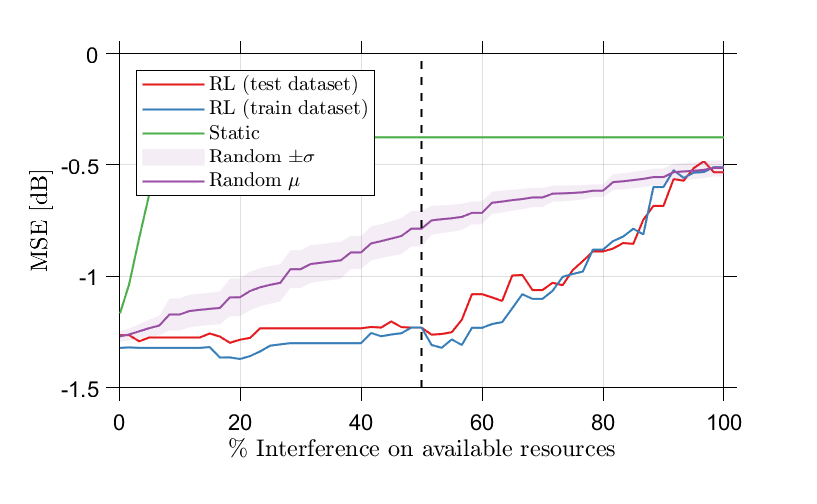
\includegraphics{chapters/part_uplink/figures/results/MSE_Interference.eps}
    \caption{Channel estimation performance (\gls{mse}) as contamination increases.}
    \label{fig:RL_MSE_Interference}
\end{figure}
In Fig. \ref{fig:RL_MSE_Interference} the \gls{mse} channel estimation performance is shown as the number of contaminated subcarriers is increased from no contamination to full bandwidth contamination. The transmitted pilot sequence span $10\%$ of the available resources. The proposed method is shown in terms of performance during training and testing. The static scheme can be seen to degrade in performance, as the number of contaminated subcarriers increases. Saturation is reached at the bandwidth of the transmitted pilot sequence ($10\%$ corresponding to $60$ subcarriers). The random scheme is shown with $\pm \sigma$. The magnitude can be seen to decrease as the amount of contaminated subcarriers increases. The training and test performance of the proposed method is shown, and the dashed line at $50\%$ contamination illustrates the dataset at which the method is trained. It can be seen that the test performance of the method is approximately constant for $0$ to $60\%$ contamination. A steady decrease in performance is observed when additional contamination is present in the radio environment. 

\begin{figure}
    \centering
    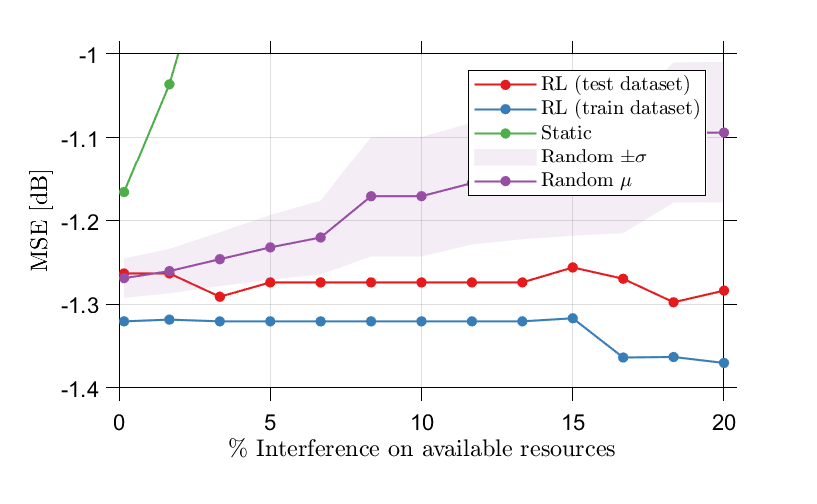
\includegraphics{chapters/part_uplink/figures/results/MSE_Interference_zoomedin.eps}
    \caption{Channel estimation performance (\gls{mse}) as contamination increases. See Fig. \ref{fig:RL_MSE_Interference}.}
    \label{fig:RL_MSE_Interference_zoomedin}
\end{figure}

When no contamination is present, the proposed method (during training) outperforms the random scheme with $0.05$ dB. however, during testing, no performance gains can be seen from $0\%$ to $5\%$, observed in Fig. \ref{fig:RL_MSE_Interference_zoomedin}. 
At $50\%$ contamination, the proposed model outperforms, the random scheme by $\approx 0.5$ dB and the static scheme by $\approx 0.9$ dB. The static scheme corresponds to doing nothing, and the performance is the effect of $5$ dB \gls{sinr} contamination. The random scheme shows a performance gain of $\approx 0.3$ dB compared to the static scheme. The performance of the proposed method reaches a minimum when full contamination is reached, or an overlap between the bandwidth of the transmitted pilot sequence and the available subcarriers that are not contaminated. Thus, from $90\%$ of contamination, the performance saturates and reaches similar values to that of the random scheme. 

\begin{figure*}
    \centering
    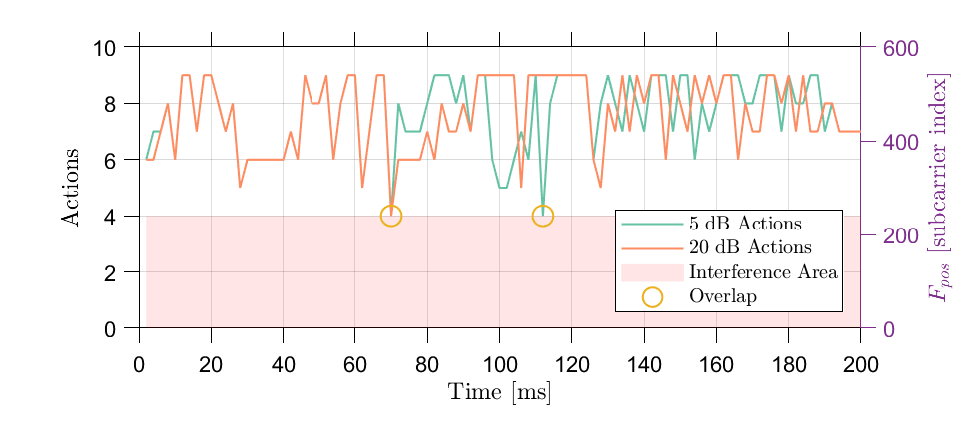
\includegraphics{chapters/part_uplink/figures/results/action_timeseries.eps}
    \caption{Actions taken over the duration of the first 200 subframes on the test set}
    \label{fig:RL_action_timeseries}
\end{figure*}

The actions taken by the algorithm for the first 200 subframes can be observed in Fig. \ref{fig:RL_action_timeseries}. It shows the area where contamination is present and where actions have been taken under the influence of $5$ dB and $20$ dB of \gls{sinr}. The taken actions enable the study of performance for higher \gls{sinr} values, as presented in Fig. \ref{fig:RL_SINR_sweep_diff}. For $5$ dB \gls{sinr}, only a single action is taken such that the \gls{srs} sequence is placed within the area of contamination. Identical behaviour is seen for $20$ dB \gls{sinr}.





\subsection{Discussion}\label{sec:RL_discussion}
The results presented in this section shows the generalised performance of the proposed approach. More specifically, as the magnitude of \gls{sinr} is varied (as presented in Section \ref{subsec:RL_results_A}), it can be seen that a near-constant level of channel estimation performance (approximately $-1.2$ dB) can be achieved regardless of the change in the magnitude of interference. It is thus indicative that the method is capable of avoiding the contaminated subcarriers, where interference is present. However, it can also be seen that the performance of the random scheme is similar (and in some cases even outperforms) the method at higher levels of \gls{sinr} (seen from $15$ to $20$ dB of \gls{sinr}). The low performance at higher levels of \gls{sinr} could indicate, that the method does not utilise information in subcarriers where contamination is present regardless of the interference magnitude. In other words, the technique does not explore the part of the spectrum where contamination is residing, even though the subcarriers contaminated contain statistical knowledge of the channel that can improve the channel estimation. The improvement of channel estimation performance using contaminated subcarriers is illustrated by the lower bound available by the random scheme (which does not care about the contamination areas or the magnitude of \gls{sinr}). At lower values of \gls{sinr}, the proposed method a performance gain of up to $0.6$ dB compared to the random scheme. 

At varying levels of contamination, i.e. interfering subcarriers (Section \ref{subsec:RL_results_B}), the method can be observed to offer nearly constant levels of performance for up to $60\%$ of the spectrum being contaminated. After which, the performance decreases almost linearly with an increase in contamination. The identical performance of the random scheme and the proposed method at $0\%$ to $5\%$ contamination does offer evidence that the proposed method can obtain no better knowledge of the channel statistics than by randomly sampling it. The gap between the training and the testing of the method does indicate that additional information is available that can improve the channel estimation. Thus, the proposed method is not capable of capturing the entirety of the channel statistics on a test set, which is evidence that the \gls{dqn} model can be further improved when observing the \gls{csi} and the actions. 

The distribution of the taken actions has been shown for different levels of \gls{sinr}. The results highlight the exploration properties of the proposed method. It is expected that the exploration increases as \gls{sinr} increases, due to the lower influence of the interference on the channel estimation performance; however, this is not the case. Similar distributions of actions (over all subframes) are observed for significant differences in levels of \gls{sinr}, which leads to believe that the method suffers from exploration issues. However, it is also the case that the model is only trained at $5$ dB of \gls{sinr} thus, it does not possess the knowledge that channel estimation can be improved at lower levels of \gls{sinr}. A solution here could be to include conditions of channel estimation error under different levels of \gls{sinr}.


\subsection{A different reward function}
\begin{figure*}
    \centering
    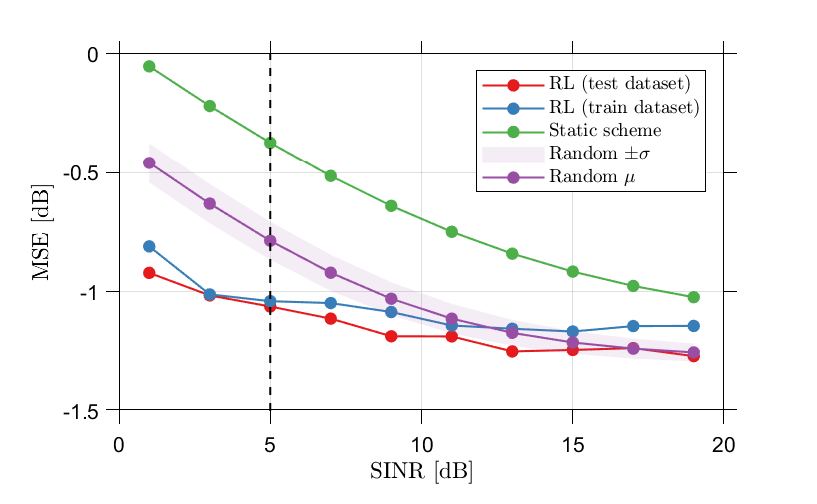
\includegraphics[width=0.5\textwidth]{chapters/part_uplink/figures/results/rewardadjustsment_-1/SINR_sweep.eps}
    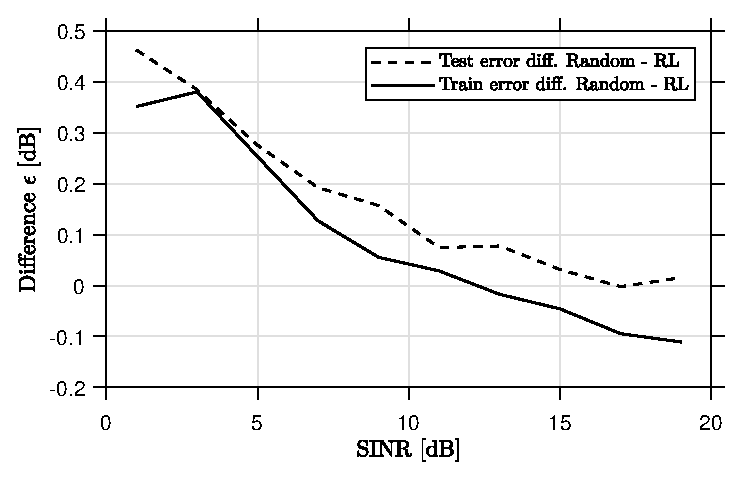
\includegraphics[width=0.45\textwidth]{chapters/part_uplink/figures/results/rewardadjustsment_-1/SINR_sweep_diff.eps}
    \caption{The performance of reward function Eq. (\ref{eq:reward_minus_1}) for different levels of \gls{sinr}}
    \label{fig:RL_different_reward_-1}
\end{figure*}

\noindent The previously presented results are obtained by using a harsh reward function, e.g. Eq. (\ref{eq:reward_minus_5}). So what happens if the reward is less harsh? A core discussion and conclusion of the present results show that the method possesses issues of exploration. In simple terms, the method avoids a penalty of $-5$ which can lead to believe that the learning is restricted. In Fig. \ref{fig:RL_different_reward_-1} the results of using a penalty of $-1$, i.e. Eq. (\ref{eq:reward_minus_1}) is used. It shows a performance increase of up to $0.5$ dB compared to the random scheme, which is less than previously shown (by $-0.1$ dB).   

The resulting action space for the first 200 subframes is shown in Fig. \ref{fig:RL_different_reward_-1_actions}. The number of actions taken in the contaminated area is increased compared to Fig. \ref{fig:RL_action_timeseries} for higher values of \gls{sinr}. Over a significant duration of the subframes, a single constant action is taken. Such behaviour can be observed from $\approx 70$ ms to $\approx 170$ ms.

\begin{figure}
    \centering
    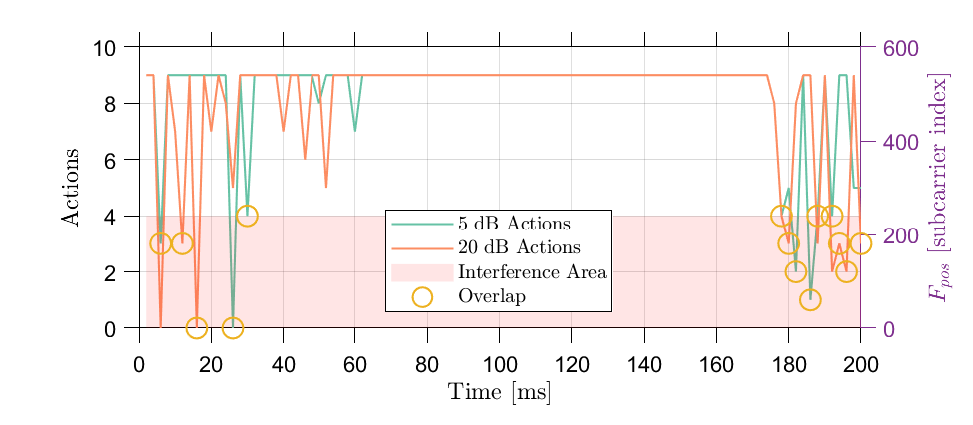
\includegraphics{chapters/part_uplink/figures/results/rewardadjustsment_-1/action_timeseries.eps}
    \caption{Actions taken for a less harsh reward function Eq. (\ref{eq:reward_minus_1})}
    \label{fig:RL_different_reward_-1_actions}
\end{figure}

The evaluation of a different reward function (with a less harsh penalty) does not result in improved performance, and on the contrary, it worsens the performance at lower levels of \gls{sinr}. Even though exploration is increased, it seems to be in vain and at the cost of being too conservative in taking actions.


\section{Discussion}
It is the purpose of the method to improve on two complex tasks related to the performance of channel estimation. Thus improve channel estimation performance by learning the channel statistics and placing pilots such that 1) interpolation accuracy is maximised, and 2) avoiding contamination. The method can be seen to be highly effective at avoiding contamination, illustrated by the near-constant channel estimation performance at both varying levels of \gls{sinr} and subcarriers influenced by contamination. These results offers evidence that the method is sufficient for providing a feasible solution for (2), so what about (1)? 

The identical performance of the method during testing and the random scheme at levels of no contamination or full contamination offers evidence that the channel statistics are not generalised, and thus the interpolation accuracy is not maximised. However, the gap between the training and the test set indicates that this is a matter of model tuning. The model is simply not extracting the necessary statistics from the raw \gls{csi} data using the \gls{dqn}. Whether this is due to ineffective learning given the reward function, or if the \gls{dqn} can be improved is left for future exploration experiments.

The computational complexity and run-time hereof is with the current implementation quite significant. A sequence of tricks of the trade (e.g. computing channel conditions offline) have been applied to speed up training. Moreover, the training have been accelerated by a GPU to further improve the conditions. Regardless of these initiatives, the training over 1000 episodes, each with 1000 subframes, takes approximately 24 hours. Such training complexity severe as a bottleneck for future advances on this subject. The channel estimator function has been identified as a root cause of the lengthy run-times. Precomputing the interpolation between the pilot signals is not possible due to it being utterly dependent on the actions taken by the method.



\section{Conclusion}\label{sec:RL_conclusion}
It has been shown that Deep Reinforcement Learning, more specifically, \gls{dqn} is capable of improving channel estimation performance through pilot placement of \gls{srs} sequences. The proposed method outperforms simple schemes that are not channel aware, by up to $0.6$ dB at low \gls{sinr}. The method can place the pilots in frequency to successfully avoid contamination parts of the spectrum. A  near-constant channel estimation error of $\approx -1.2$ dB using a linear channel estimator is achieved from $0$ to $20$ dB of \gls{sinr} with a slight performance increasing trend as \gls{sinr} increases. Varying the amount of contamination present in the spectrum (not only the magnitude but also the span of subcarriers) provides a constant channel estimation error (of also $\approx -1.2$ dB) for up to $60\%$ of the spectrum. Subsequent, a slight decrease of performance is seen until the bandwidth spanned by the \gls{srs} pilot sequence, e.g. $90 \%$ of the spectrum contaminated. 

The proposed method is capable of obtaining channel statistics that can improve the interpolation function of the channel estimator, however with a few caveats. A channel estimation performance gain of $0.05$ dB is reported comparing to randomly sampled subcarriers of the spectrum. Finally, A generalisation gap between training and testing is reported and identified as a sub-optimal training routine related to one of two core issues, 1) exploration imposed by the reward function and 2) information bottleneck when observing the raw \gls{csi}.

\section{Identified challenges}\label{sec:RL_challenges}
A method for placing \gls{srs} sequences in uplink using Deep Reinforcement Learning has been documented in this chapter. Channel estimation gains have been shown for different configurations of contamination. The results, discussion and conclusion, has contributed towards a more intelligent cellular system where pilot contamination can be mitigated using learned models. A few challenges have been identified along the way, and can be reduced to the following essential points:

\begin{itemize}
    \item Exploration of reinforcement learning actions does not equal improved performance.
    \item Computational complexity is a major bottleneck for further advances.
    \item Fundamental changes, such as user velocities and delay spread, to the channel characteristics, is largely untested.
    \item The current reward function based on channel estimation performance is not practically feasible.
\end{itemize}


\section{Summary}\label{sec:RL_summary}
Processing \gls{ofdm} symbols of received \gls{csi} using image processing techniques is beneficial for self-learning reinforcement learning systems. The Deep Reinforcement Learning algorithm is shown to be capable of learning how pilot placement affects the resulting channel estimation performance. The proposed method is capable of avoiding pilot contamination sources. The method learns the necessary mapping between a pilot placement and the observed \gls{csi} in order to deduce the best future pilot placement effectively. The feasibility of using such a method in mobile communication systems have been discussed. The method is capable of operating completely autonomous and therefore require no complex data set engineering unlike the supervised techniques as presented in chapter \ref{ch:channel_estimation}. The lower data requirements reduce the implementation bottleneck and highlight the feasibility of a Deep Reinforcement Learning application in future cellular networks. The specific outcome of the above-detailed method can be summarised as follows

\begin{itemize}
    \item Deep Q-Learning algorithms are effective at learning improved \gls{srs} sequence placement from observed \gls{csi}. 
    \item The proposed method can actively avoid unknown contamination sources by interacting with the radio environment. 
    \item Deep Reinforcement Learning is subject to improved implementations for use in mobile communication system research. 
\end{itemize}

